% Drawing 142/04-2 -- folder 142, batch 04, archive page 63 (PDF page 64).
% Transcription: En marge gauche : deux petits cercles, aux points $R^{\omega}_{\omega i}$ et $R^{\omega'}_{\omega' i}$, joints par un chemin fléché $\widetilde{b}_i^{\omega}$ qui passe par $Q_i$.
% Kind: path between two small circles. Method 2 (schematic redraw from the facsimile). Status: ok.
% Notes: Two small circles at R^omega_{omega i} (left) and R^{omega'}_{omega' i} (right, cut by the edge of the drawing), joined by the thick path tilde b_i^omega through Q_i. No arrowhead is legible on the page; none is drawn.
% Coordinates: 1 unit = 1 mm = 1/100 of the crop width (bbox in page fractions: [0.1, 0.5, 0.32, 0.57]).
% Redrawn by Claude (claude-opus-5-5), issue #73, 2026-11-07; not checked by a human; not compiled (no TeX in the session).
% Rights: reproduces part of the work -- behind RENDER_TRANSCRIPTS, never published by itself.
\documentclass[tikz,border=3pt]{standalone}
\usepackage{amsmath,amssymb}
\usetikzlibrary{patterns,arrows.meta}
\tikzset{pencil/.style={black!45}, struck/.style={black!35}, mark/.style={circle,draw,inner sep=1.3pt}, pt/.style={circle,fill,inner sep=0.9pt}, opt/.style={circle,draw,fill=white,inner sep=1.1pt}}
\begin{document}
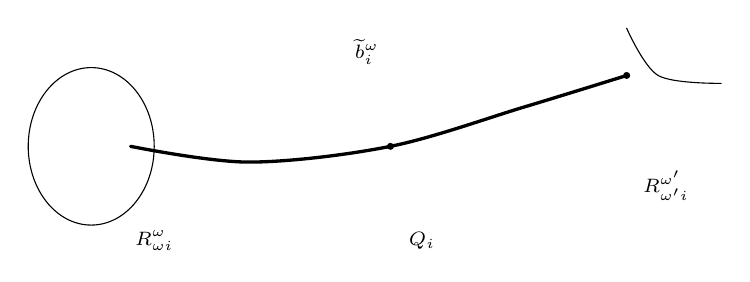
\begin{tikzpicture}[x=1mm,y=1mm,line cap=round,line join=round,font=\scriptsize]
\draw (20,-18) ellipse[x radius=8, y radius=10];
\draw[very thick] plot[smooth, tension=0.55] coordinates {(25,-18) (40,-20) (58,-18) (75,-13) (88,-9)};
\node[pt] at (58,-18) {};
\node[pt] at (88,-9) {};
\draw plot[smooth, tension=0.55] coordinates {(88,-3) (92,-9) (100,-10)};
\node[inner sep=1pt] at (28,-30) {\scriptsize $R^{\omega}_{\omega i}$};
\node[inner sep=1pt] at (55,-6) {\scriptsize $\widetilde b_i^{\omega}$};
\node[inner sep=1pt] at (62,-30) {\scriptsize $Q_i$};
\node[inner sep=1pt] at (93,-23) {\scriptsize $R^{\omega'}_{\omega' i}$};
\end{tikzpicture}
\end{document}
